\documentclass[11pt]{article}

\usepackage[a4paper,margin=1in]{geometry}
\usepackage[T1]{fontenc}
\usepackage[utf8]{inputenc}
\usepackage{lmodern}
\usepackage{amsmath,amssymb,amsthm,mathtools}
\usepackage{enumitem}
\usepackage{hyperref}
\usepackage{microtype}
\usepackage{graphicx}
\usepackage{caption}
\usepackage{booktabs}
\usepackage{float}
\usepackage[section]{placeins}
\usepackage{algorithm}
\usepackage{algpseudocode}
\captionsetup{font=small}

\hypersetup{
    hidelinks
}

\newtheorem{theorem}{Theorem}[section]
\newtheorem{proposition}[theorem]{Proposition}
\newtheorem{lemma}[theorem]{Lemma}
\newtheorem{corollary}[theorem]{Corollary}
\theoremstyle{definition}
\newtheorem{definition}[theorem]{Definition}
\newtheorem{assumption}[theorem]{Assumption}
\theoremstyle{remark}
\newtheorem{remark}[theorem]{Remark}

\newcommand{\R}{\mathbb{R}}
\newcommand{\X}{\mathcal{X}}
\newcommand{\E}{\mathbb{E}}
\newcommand{\inner}[2]{\langle #1, #2 \rangle}
\newcommand{\norm}[1]{\lVert #1 \rVert}
\newcommand{\normdual}[1]{\lVert #1 \rVert_*}
\DeclareMathOperator*{\argmin}{arg\,min}
\DeclareMathOperator*{\argmax}{arg\,max}
\DeclareMathOperator{\dom}{dom}

\title{A Generalized Approach to Nonsmooth Convex Optimization}
\author{Xiangyu LUO}
\date{April 2026}

\begin{document}

\maketitle

\tableofcontents

\section{Introduction}
Let $f : \R^d \to \R$ be a convex function and let $\X \subset \R^d$ be a nonempty closed convex set. We consider the constrained problem
\[
    \min_{x \in \X} f(x),
\]
which we assume admits a minimizer $x^* \in \X$. The report studies a generalized weighted-averaging framework in which, given a sequence $(x_t)_{t\ge 1}$ in $\R^d$, a positive weight sequence $(\gamma_t)_{t\ge 1}$, and an interpolation sequence $(\beta_t)_{t\ge 1} \subset [0,1]$ and evaluates the subgradient at the interpolated point, $g_t \in \partial f(z_t)$. The goal is to bound the optimization gap $f(\bar{x}_T)-f(x^*)$ at the weighted average.

The report follows the five questions of the assignment. Section~\ref{sec:monotonicity} proves monotonicity of convex subgradients (Question~1). Section~\ref{sec:averaging} proves the averaging identities, the one-step descent inequality, and the ergodic bound on $f(\bar{x}_T)-f(x^*)$ (Question~2, parts a--c). Section~\ref{sec:deterministic} addresses Question~3: under an $L$-Lipschitz assumption, it instantiates the ergodic bound for mirror descent, projected subgradient descent, dual averaging with time-dependent parameters, and AdaGrad-Norm, and derives explicit guarantees. Section~\ref{sec:stochastic} extends these guarantees to the stochastic setting, where the subgradient is replaced by a conditionally unbiased estimator with bounded second moment (Question~4). Section~\ref{sec:experiments} reports numerical experiments on SVM and related benchmarks, comparing various choices of $(\gamma_t)_{t\ge 1}$ and $(\beta_t)_{t\ge 1}$ (Question~5).

\section{Mathematical proofs and derivations}

Let $(x_t)_{t\ge 1}$ be a sequence in $\R^d$, let $(\gamma_t)_{t\ge 1}$ be a positive sequence, and let $(\beta_t)_{t\ge 1}$ be a sequence in $[0,1]$. For every $t\ge 1$, define
\[
    \Gamma_t = \sum_{s=1}^t \gamma_s,
    \qquad
    \bar{x}_t = \frac{1}{\Gamma_t}\sum_{s=1}^t \gamma_s x_s,
    \qquad
    z_t = \beta_t \bar{x}_t + (1-\beta_t)x_t,
\]
and choose $g_t \in \partial f(z_t)$. Since $f$ is real-valued and convex on all of $\R^d$, its subdifferential is nonempty at every point, so this choice is legitimate. We also set $\Gamma_0 := 0$ and interpret $\Gamma_0 f(\bar{x}_0)$ as zero, so no explicit value of $\bar{x}_0$ is needed.

\subsection{Monotonicity of convex subgradients}
\label{sec:monotonicity}

\begin{proposition}[Monotonicity of convex subgradients]
\label{prop:monotonicity}
For all $x,x' \in \R^d$, for all $y \in \partial f(x)$ and $y' \in \partial f(x')$, one has
\[
    \inner{y'-y}{x'-x} \ge 0.
\]
\end{proposition}

\begin{proof}
Since $y \in \partial f(x)$ and $y' \in \partial f(x')$, the subgradient inequalities are
\[
    f(x') \ge f(x) + \inner{y}{x'-x}
    \qquad\text{and}\qquad
    f(x) \ge f(x') + \inner{y'}{x-x'}.
\]
Adding them gives
\[
    0 \ge \inner{y-y'}{x'-x},
\]
which is equivalent to the claimed inequality.
\end{proof}

\subsubsection{Weighted averaging identities}
\label{sec:averaging}

\begin{lemma}[Weighted averaging identities]
\label{lem:averaging-identities}
For every $t\ge 2$,
\[
    \bar{x}_t - \bar{x}_{t-1} = \frac{\gamma_t}{\Gamma_{t-1}}(x_t-\bar{x}_t).
\]
Moreover, for every $t\ge 1$ such that $\beta_t<1$,
\[
    x_t-z_t = \frac{\beta_t}{1-\beta_t}(z_t-\bar{x}_t).
\]
\end{lemma}

\begin{proof}
Fix $t\ge 2$. By definition,
\[
    \Gamma_t \bar{x}_t
    =
    \sum_{s=1}^t \gamma_s x_s
    =
    \Gamma_{t-1}\bar{x}_{t-1} + \gamma_t x_t.
\]
Since $\Gamma_t = \Gamma_{t-1}+\gamma_t$, we obtain
\[
    (\Gamma_{t-1}+\gamma_t)\bar{x}_t
    =
    \Gamma_{t-1}\bar{x}_{t-1} + \gamma_t x_t.
\]
After rearranging,
\[
    \Gamma_{t-1}(\bar{x}_t-\bar{x}_{t-1}) = \gamma_t(x_t-\bar{x}_t),
\]
and division by $\Gamma_{t-1}>0$ gives the first identity.

For the second identity, the definition of $z_t$ yields
\[
    x_t-z_t = x_t-\beta_t\bar{x}_t-(1-\beta_t)x_t = \beta_t(x_t-\bar{x}_t),
\]
whereas
\[
    z_t-\bar{x}_t = \beta_t\bar{x}_t + (1-\beta_t)x_t-\bar{x}_t = (1-\beta_t)(x_t-\bar{x}_t).
\]
If $\beta_t<1$, one has $x_t-\bar{x}_t = (z_t-\bar{x}_t)/(1-\beta_t)$, and substituting this into the first identity gives the result.
\end{proof}

\begin{remark}
\label{rem:beta-one}
When $\beta_t=1$, one has $z_t=\bar{x}_t$. The second identity in Lemma~\ref{lem:averaging-identities} is then unnecessary.
\end{remark}

\subsubsection{One-step inequality and ergodic bound}

\begin{proposition}[One-step descent inequality]
\label{prop:one-step}
For every $t\ge 1$,
\[
    \Gamma_t f(\bar{x}_t) - \Gamma_{t-1}f(\bar{x}_{t-1}) - \gamma_t f(x^*)
    \le
    \inner{\gamma_t g_t}{x_t-x^*}.
\]
\end{proposition}

\begin{proof}
For $t=1$, one has $\bar{x}_1=x_1$ and therefore $z_1=x_1$. Since $g_1 \in \partial f(x_1)$,
\[
    \Gamma_1 f(\bar{x}_1)-\Gamma_0 f(\bar{x}_0)-\gamma_1 f(x^*)
    =
    \gamma_1\bigl(f(x_1)-f(x^*)\bigr)
    \le
    \inner{\gamma_1 g_1}{x_1-x^*}.
\]

Now fix $t\ge 2$ and choose $\tilde g_t \in \partial f(\bar{x}_t)$. Write
\begin{align*}
    &\Gamma_t f(\bar{x}_t)-\Gamma_{t-1}f(\bar{x}_{t-1})-\gamma_t f(x^*) \\
    &\qquad =
    \Gamma_{t-1}\bigl(f(\bar{x}_t)-f(\bar{x}_{t-1})\bigr)
    +
    \gamma_t\bigl(f(\bar{x}_t)-f(z_t)\bigr)
    +
    \gamma_t\bigl(f(z_t)-f(x^*)\bigr).
\end{align*}
The subgradient inequality gives
\[
    f(\bar{x}_t)-f(\bar{x}_{t-1}) \le \inner{\tilde g_t}{\bar{x}_t-\bar{x}_{t-1}},
    \qquad
    f(\bar{x}_t)-f(z_t) \le \inner{\tilde g_t}{\bar{x}_t-z_t},
\]
and
\[
    f(z_t)-f(x^*) \le \inner{g_t}{z_t-x^*}.
\]
Hence
\begin{align*}
    &\Gamma_t f(\bar{x}_t)-\Gamma_{t-1}f(\bar{x}_{t-1})-\gamma_t f(x^*) \\
    &\qquad \le
    \Gamma_{t-1}\inner{\tilde g_t}{\bar{x}_t-\bar{x}_{t-1}}
    +
    \gamma_t\inner{\tilde g_t}{\bar{x}_t-z_t}
    +
    \gamma_t\inner{g_t}{z_t-x^*}.
\end{align*}
By Lemma~\ref{lem:averaging-identities},
\[
    \Gamma_{t-1}(\bar{x}_t-\bar{x}_{t-1}) = \gamma_t(x_t-\bar{x}_t),
\]
so the first two terms combine into
\[
    \gamma_t\inner{\tilde g_t}{x_t-\bar{x}_t}
    +
    \gamma_t\inner{\tilde g_t}{\bar{x}_t-z_t}
    =
    \gamma_t\inner{\tilde g_t}{x_t-z_t}.
\]
Therefore,
\[
    \Gamma_t f(\bar{x}_t)-\Gamma_{t-1}f(\bar{x}_{t-1})-\gamma_t f(x^*)
    \le
    \gamma_t\inner{\tilde g_t}{x_t-z_t}
    +
    \gamma_t\inner{g_t}{z_t-x^*}.
\]

If $\beta_t<1$, Proposition~\ref{prop:monotonicity} applied to $(\bar{x}_t,\tilde g_t)$ and $(z_t,g_t)$ yields
\[
    \inner{g_t-\tilde g_t}{z_t-\bar{x}_t} \ge 0.
\]
By Lemma~\ref{lem:averaging-identities}, $x_t-z_t$ is a nonnegative multiple of $z_t-\bar{x}_t$, hence
\[
    \inner{\tilde g_t-g_t}{x_t-z_t} \le 0,
    \qquad
    \inner{\tilde g_t}{x_t-z_t} \le \inner{g_t}{x_t-z_t}.
\]
Substituting this into the previous bound yields
\[
    \Gamma_t f(\bar{x}_t)-\Gamma_{t-1}f(\bar{x}_{t-1})-\gamma_t f(x^*)
    \le
    \gamma_t\inner{g_t}{x_t-z_t}
    +
    \gamma_t\inner{g_t}{z_t-x^*}
    =
    \gamma_t\inner{g_t}{x_t-x^*}.
\]

If $\beta_t=1$, then $z_t=\bar{x}_t$; taking $\tilde g_t=g_t$ gives the same conclusion.
\end{proof}

\begin{theorem}[Ergodic optimization bound]
\label{thm:ergodic}
For every $T\ge 1$,
\[
    f(\bar{x}_T)-f(x^*)
    \le
    \frac{1}{\Gamma_T}\sum_{t=1}^T \inner{\gamma_t g_t}{x_t-x^*}.
\]
\end{theorem}

\begin{proof}
Summing Proposition~\ref{prop:one-step} over $t=1,\dots,T$ gives
\[
    \sum_{t=1}^T
    \Bigl(
        \Gamma_t f(\bar{x}_t)-\Gamma_{t-1}f(\bar{x}_{t-1})-\gamma_t f(x^*)
    \Bigr)
    \le
    \sum_{t=1}^T \inner{\gamma_t g_t}{x_t-x^*}.
\]
The left-hand side telescopes to
\[
    \Gamma_T f(\bar{x}_T) - \sum_{t=1}^T \gamma_t f(x^*)
    =
    \Gamma_T\bigl(f(\bar{x}_T)-f(x^*)\bigr).
\]
Since $\sum_{t=1}^T \gamma_t = \Gamma_T$, division by $\Gamma_T$ yields the result.
\end{proof}

\subsection{Deterministic nonsmooth convex optimization}
\label{sec:deterministic}

From now on, the algorithms are constrained to $\X$, so $x_t \in \X$ for every $t$. Since $\X$ is convex, this implies $\bar{x}_t, z_t \in \X$ for all $t\ge 1$.

Let $\norm{\cdot}$ be a norm on $\R^d$ and assume that $f$ is $L$-Lipschitz continuous with respect to $\norm{\cdot}$. Because $f$ is convex on all of $\R^d$, every subgradient of $f$ satisfies $\normdual{g} \le L$.

A \emph{regularizer} is a proper, strictly convex, lower semicontinuous function $h : \R^d \to \R \cup \{+\infty\}$ such that $\dom h^*=\R^d$. Whenever such a function is used on the constrained set $\X$, we assume $\dom h \subseteq \X$.

A \emph{mirror map compatible with $\X$} is a function $H : \R^d \to \R \cup \{+\infty\}$ such that, with $D_H := \operatorname{int}(\dom H)$,
\begin{enumerate}[label=(\roman*)]
    \item $H$ is lower semicontinuous, strictly convex, and differentiable on $D_H$;
    \item $\nabla H(D_H)=\R^d$;
    \item $\X \subseteq \operatorname{cl}(D_H)$;
    \item $\X \cap D_H \neq \varnothing$.
\end{enumerate}
For $x \in \dom h$, $x' \in \R^d$, and $y \in \partial h(x)$, the generalized Bregman divergence is defined by
\[
    D_h(x',x;y) = h(x')-h(x)-\inner{y}{x'-x}.
\]
If $H$ is differentiable at $x$, this reduces to the usual Bregman divergence
\[
    D_H(x',x) = H(x')-H(x)-\inner{\nabla H(x)}{x'-x}.
\]

\begin{proposition}[Transfer from regret to optimization]
\label{prop:transfer}
Assume that an online linear optimization method produces iterates $x_t \in \X$ and satisfies, for every $x \in \X$,
\[
    \sum_{t=1}^T \inner{u_t}{x-x_t} \le \mathrm{Reg}_T(x).
\]
If the method is fed with payoff vectors $u_t = -\gamma_t g_t$, where $g_t \in \partial f(z_t)$, then
\[
    f(\bar{x}_T)-f(x^*)
    \le
    \frac{\mathrm{Reg}_T(x^*)}{\Gamma_T}.
\]
\end{proposition}

\begin{proof}
With $u_t=-\gamma_t g_t$, the regret inequality becomes
\[
    \sum_{t=1}^T \inner{\gamma_t g_t}{x_t-x} \le \mathrm{Reg}_T(x)
    \qquad (x \in \X).
\]
Taking $x=x^*$ and invoking Theorem~\ref{thm:ergodic} yields
\[
    f(\bar{x}_T)-f(x^*)
    \le
    \frac{1}{\Gamma_T}\sum_{t=1}^T \inner{\gamma_t g_t}{x_t-x^*}
    \le
    \frac{\mathrm{Reg}_T(x^*)}{\Gamma_T}.
\]
\end{proof}

\subsubsection{Mirror descent and projected subgradient descent}

\begin{proposition}[Weighted-average mirror descent]
\label{prop:mirror-descent}
Let $H$ be a mirror map compatible with $\X$, assume that $H$ is $K$-strongly convex with respect to $\norm{\cdot}$, let $x_1 \in \X \cap \operatorname{int}(\dom H)$, and assume that $x^* \in \X \cap \dom H$. Consider the update
\[
    x_{t+1}
    =
    \argmin_{x \in \X}
    \left\{
        \inner{\gamma_t g_t}{x}
        +
        D_H(x,x_t)
    \right\},
    \qquad
    g_t \in \partial f(z_t).
\]
Then, for every $T\ge 1$,
\[
    f(\bar{x}_T)-f(x^*)
    \le
    \frac{D_H(x^*,x_1) + \frac{1}{2K}\sum_{t=1}^T \gamma_t^2\normdual{g_t}^2}{\Gamma_T}.
\]
In particular, if
\[
    \gamma_t = \frac{\gamma \sqrt{2K}}{L\sqrt{t}},
\]
then
\[
    f(\bar{x}_T)-f(x^*)
    \le
    \frac{L}{\sqrt{2KT}}
    \left(
        \frac{D_H(x^*,x_1)}{\gamma}
        +
        \gamma(1+\log T)
    \right).
\]
If, moreover, $D_H(x^*,x_1)\le R^2$ and $\gamma=R$, then
\[
    f(\bar{x}_T)-f(x^*) 
    \le
    \frac{RL(2+\log T)}{\sqrt{2KT}}.
\]
\end{proposition}

\begin{proof}
Because $H$ is a compatible mirror map and $x_t \in \X \cap \operatorname{int}(\dom H)$, the minimizer $x_{t+1}$ also belongs to $\X \cap \operatorname{int}(\dom H)$.

For every $t\ge 1$, the optimality condition of the update yields
\[
    \inner{\gamma_t g_t + \nabla H(x_{t+1})-\nabla H(x_t)}{x-x_{t+1}} \ge 0
    \qquad
    (x \in \X).
\]
By the three-point identity for Bregman divergences,
\[
    \inner{\gamma_t g_t}{x_{t+1}-x}
    \le
    D_H(x,x_t)-D_H(x,x_{t+1})-D_H(x_{t+1},x_t).
\]
Taking $x=x^*$ and adding $\inner{\gamma_t g_t}{x_t-x_{t+1}}$ to both sides gives
\[
    \inner{\gamma_t g_t}{x_t-x^*}
    \le
    D_H(x^*,x_t)-D_H(x^*,x_{t+1})-D_H(x_{t+1},x_t)
    +
    \inner{\gamma_t g_t}{x_t-x_{t+1}}.
\]
Since $H$ is $K$-strongly convex,
\[
    D_H(x_{t+1},x_t) \ge \frac{K}{2}\norm{x_{t+1}-x_t}^2.
\]
Young's inequality yields
\[
    \inner{\gamma_t g_t}{x_t-x_{t+1}}
    \le
    \frac{\gamma_t^2}{2K}\normdual{g_t}^2
    +
    \frac{K}{2}\norm{x_t-x_{t+1}}^2,
\]
whence
\[
    \inner{\gamma_t g_t}{x_t-x^*}
    \le
    D_H(x^*,x_t)-D_H(x^*,x_{t+1})
    +
    \frac{\gamma_t^2}{2K}\normdual{g_t}^2.
\]
Summing over $t=1,\dots,T$ gives
\[
    \sum_{t=1}^T \inner{\gamma_t g_t}{x_t-x^*}
    \le
    D_H(x^*,x_1)
    +
    \frac{1}{2K}\sum_{t=1}^T \gamma_t^2\normdual{g_t}^2.
\]
Therefore, Theorem~\ref{thm:ergodic} gives
\[
    f(\bar{x}_T)-f(x^*)
    \le
    \frac{D_H(x^*,x_1) + \frac{1}{2K}\sum_{t=1}^T \gamma_t^2\normdual{g_t}^2}{\Gamma_T}.
\]
Since $\normdual{g_t}\le L$, the choice $\gamma_t = \gamma\sqrt{2K}/(L\sqrt{t})$ yields
\[
    \frac{1}{2K}\sum_{t=1}^T \gamma_t^2\normdual{g_t}^2
    \le
    \gamma^2\sum_{t=1}^T \frac{1}{t}
    \le
    \gamma^2(1+\log T).
\]
Moreover,
\[
    \Gamma_T
    =
    \frac{\gamma\sqrt{2K}}{L}\sum_{t=1}^T \frac{1}{\sqrt{t}}
    \ge
    \frac{\gamma\sqrt{2KT}}{L}.
\]
Substituting these bounds proves the displayed estimate. The last claim follows by setting $\gamma=R$.
\end{proof}

\begin{corollary}[Weighted-average projected subgradient method]
\label{cor:euclidean-md}
Assume that $\X \subset \R^d$ is equipped with the Euclidean norm and consider
\[
    x_{t+1} = \Pi_{\X}(x_t-\gamma_t g_t),
    \qquad
    g_t \in \partial f(z_t).
\]
If $f$ is $L$-Lipschitz with respect to $\norm{\cdot}_2$ and
\[
    \gamma_t = \frac{\gamma\sqrt{2}}{L\sqrt{t}},
\]
then, for every $T\ge 1$,
\[
    f(\bar{x}_T)-f(x^*)
    \le
    \frac{L}{\sqrt{2T}}
    \left(
        \frac{\norm{x^*-x_1}_2^2}{2\gamma}
        +
        \gamma(1+\log T)
    \right).
\]
If $\frac12 \norm{x^*-x_1}_2^2 \le R^2$ and $\gamma=R$, then
\[
    f(\bar{x}_T)-f(x^*)
    \le
    \frac{RL(2+\log T)}{\sqrt{2T}}.
\]
\end{corollary}

\begin{proof}
Take $H(x)=\tfrac12 \norm{x}_2^2$ in Proposition~\ref{prop:mirror-descent}. Then $H$ is $1$-strongly convex, the update becomes
\[
    x_{t+1} = \Pi_{\X}(x_t-\gamma_t g_t),
\]
and
\[
    D_H(x^*,x_1) = \frac12 \norm{x^*-x_1}_2^2.
\]
Substituting these identities gives the result.
\end{proof}

\subsubsection{Dual averaging with time-dependent parameters}

\begin{proposition}[Weighted-average dual averaging]
\label{prop:dual-averaging}
Let $h$ be a regularizer, assume that $h$ is $K$-strongly convex with respect to $\norm{\cdot}$, let $x^* \in \dom h$, and define
\[
    x_t = \nabla h^*\!\left(-\eta_t \sum_{s=1}^{t-1} g_s\right),
    \qquad
    t\ge 1,
\]
where $g_t \in \partial f(z_t)$ and $(\eta_t)_{t\ge 1}$ is positive and nonincreasing. Let $\gamma_t=1$, so that $\Gamma_T=T$ and $\bar{x}_T = T^{-1}\sum_{t=1}^T x_t$. Then, for every $T\ge 1$,
\[
    \sum_{t=1}^T \inner{g_t}{x_t-x^*}
    \le
    \frac{h(x^*)-\min h}{\eta_T}
    +
    \frac{1}{2K}\sum_{t=1}^T \eta_t \normdual{g_t}^2,
\]
and therefore
\[
    f(\bar{x}_T)-f(x^*)
    \le
    \frac{1}{T}
    \left(
        \frac{h(x^*)-\min h}{\eta_T}
        +
        \frac{1}{2K}\sum_{t=1}^T \eta_t \normdual{g_t}^2
    \right).
\]
If, moreover,
\[
    \eta_t = \frac{\eta\sqrt{K}}{L\sqrt{t}},
\]
then
\[
    f(\bar{x}_T)-f(x^*)
    \le
    \left(
        \frac{h(x^*)-\min h}{\eta}
        +
        \eta
    \right)
    \frac{L}{\sqrt{KT}}.
\]
If $h(x^*)-\min h \le R^2$ and $\eta=R$, then
\[
    f(\bar{x}_T)-f(x^*) \le \frac{2LR}{\sqrt{KT}}.
\]
\end{proposition}

\begin{proof}
Set $y_1=0$ and $y_{t+1}=y_t-g_t$. Then
\[
    x_t = \nabla h^*(\eta_t y_t),
\]
so this is the dual-averaging scheme with time-dependent parameter $\eta_t$. The corresponding regret bound for dual averaging with time-dependent parameters gives
\[
    \sum_{t=1}^T \inner{g_t}{x_t-x^*}
    \le
    \frac{h(x^*)-\min h}{\eta_T}
    +
    \frac{1}{2K}\sum_{t=1}^T \eta_t \normdual{g_t}^2.
\]
The objective bound then follows from Theorem~\ref{thm:ergodic}, because $\gamma_t=1$ for all $t$.

For the choice $\eta_t = \eta\sqrt{K}/(L\sqrt{t})$, one has
\[
    \frac{h(x^*)-\min h}{\eta_T}
    =
    \frac{h(x^*)-\min h}{\eta}\,L\sqrt{\frac{T}{K}},
\]
and, since $\normdual{g_t}\le L$,
\[
    \frac{1}{2K}\sum_{t=1}^T \eta_t \normdual{g_t}^2
    \le
    \frac{L^2}{2K}\sum_{t=1}^T \eta_t
    \le
    \eta L\sqrt{\frac{T}{K}},
\]
where we used $\sum_{t=1}^T t^{-1/2} \le 2\sqrt{T}$. Dividing by $T$ gives the claimed estimate. The last conclusion follows by setting $\eta=R$.
\end{proof}

\subsubsection{AdaGrad-Norm}

\begin{proposition}[Weighted-average AdaGrad-Norm]
\label{prop:adagrad}
Assume that $\X \subset \R^d$ is equipped with the Euclidean norm, choose $\gamma_t=1$, and consider
\[
    x_{t+1}
    =
    \Pi_{\X}\left(
        x_t - \frac{\gamma}{\sqrt{\sum_{s=1}^t \norm{g_s}_2^2}}\,g_t
    \right),
    \qquad
    g_t \in \partial f(z_t),
\]
with the convention $0/0=0$. Then, for every $T\ge 1$,
\[
    f(\bar{x}_T)-f(x^*)
    \le
    \frac{1}{T}
    \left(
        \frac{\max_{1\le t\le T} \norm{x_t-x^*}_2^2}{2\gamma} + \gamma
    \right)
    \sqrt{\sum_{t=1}^T \norm{g_t}_2^2}.
\]
If, in addition,
\[
    \max_{1\le t\le T} \norm{x_t-x^*}_2 \le R,
\]
then
\[
    f(\bar{x}_T)-f(x^*)
    \le
    \left(
        \frac{R^2}{2\gamma} + \gamma
    \right)\frac{L}{\sqrt{T}}.
\]
Choosing $\gamma = R/\sqrt{2}$ gives
\[
    f(\bar{x}_T)-f(x^*) \le RL\sqrt{\frac{2}{T}}.
\]
\end{proposition}

\begin{proof}
The pathwise regret bound for AdaGrad-Norm yields
\[
    \sum_{t=1}^T \inner{g_t}{x_t-x^*}
    \le
    \left(
        \frac{\max_{1\le t\le T} \norm{x_t-x^*}_2^2}{2\gamma} + \gamma
    \right)
    \sqrt{\sum_{t=1}^T \norm{g_t}_2^2}.
\]
Since $\gamma_t=1$, Theorem~\ref{thm:ergodic} gives the first bound. If $\max_{1\le t\le T} \norm{x_t-x^*}_2 \le R$, then
\[
    \sqrt{\sum_{t=1}^T \norm{g_t}_2^2} \le L\sqrt{T}.
\]
Whence the second estimate follows. The choice $\gamma = R/\sqrt{2}$ minimizes the prefactor.
\end{proof}

\subsection{Stochastic nonsmooth convex optimization}
\label{sec:stochastic}

Let $(\mathcal{F}_t)_{t\ge 0}$ be a filtration. Assume that $x_t$ and $z_t$ are $\mathcal{F}_{t-1}$-measurable for every $t\ge 1$. Let $G_t$ be a random estimator such that
\[
    \E[G_t \mid \mathcal{F}_{t-1}] \in \partial f(z_t)
    \quad\text{a.s.},
    \qquad
    \E[\normdual{G_t}^2 \mid \mathcal{F}_{t-1}] \le \sigma^2
    \quad\text{a.s.}
\]
for some $\sigma>0$.

\begin{proposition}[Stochastic transfer]
\label{prop:stochastic-transfer}
Under the preceding assumptions,
\[
    \E[f(\bar{x}_T)-f(x^*)]
    \le
    \frac{1}{\Gamma_T}
    \E\left[
        \sum_{t=1}^T \inner{\gamma_t G_t}{x_t-x^*}
    \right].
\]
\end{proposition}

\begin{proof}
Define $\widehat g_t = \E[G_t \mid \mathcal{F}_{t-1}]$. Then $\widehat g_t \in \partial f(z_t)$ almost surely. Applying Theorem~\ref{thm:ergodic} pathwise to the sequences $(x_t,z_t,\widehat g_t)$ gives
\[
    f(\bar{x}_T)-f(x^*)
    \le
    \frac{1}{\Gamma_T}\sum_{t=1}^T \inner{\gamma_t \widehat g_t}{x_t-x^*}
    \qquad \text{a.s.}
\]
Taking expectations and using the tower property yields
\[
    \E\bigl[\inner{\gamma_t \widehat g_t}{x_t-x^*}\bigr]
    =
    \E\!\left[
        \E\!\left[\inner{\gamma_t G_t}{x_t-x^*} \,\middle|\, \mathcal{F}_{t-1}\right]
    \right]
    =
    \E\bigl[\inner{\gamma_t G_t}{x_t-x^*}\bigr],
\]
which proves the claim.
\end{proof}

\subsubsection{Stochastic mirror descent}

\begin{proposition}[Weighted-average stochastic mirror descent]
\label{prop:stochastic-md}
Let $H$ be a mirror map compatible with $\X$, assume that $H$ is $K$-strongly convex with respect to $\norm{\cdot}$, let $x_1 \in \X \cap \operatorname{int}(\dom H)$, and assume that $x^* \in \X \cap \dom H$. Define
\[
    x_{t+1}
    =
    \argmin_{x \in \X}
    \left\{
        \inner{\gamma_t G_t}{x}
        +
        D_H(x,x_t)
    \right\}.
\]
Then
\[
    \E\left[
        \sum_{t=1}^T \inner{\gamma_t G_t}{x_t-x^*}
    \right]
    \le
    D_H(x^*,x_1)
    +
    \frac{\sigma^2}{2K}\sum_{t=1}^T \gamma_t^2,
\]
and therefore
\[
    \E[f(\bar{x}_T)-f(x^*)]
    \le
    \frac{D_H(x^*,x_1) + \frac{\sigma^2}{2K}\sum_{t=1}^T \gamma_t^2}{\Gamma_T}.
\]
If
\[
    \gamma_t = \frac{\gamma \sqrt{2K}}{\sigma\sqrt{t}},
\]
then
\[
    \E[f(\bar{x}_T)-f(x^*)]
    \le
    \frac{\sigma}{\sqrt{2KT}}
    \left(
        \frac{D_H(x^*,x_1)}{\gamma}
        +
        \gamma(1+\log T)
    \right).
\]
\end{proposition}

\begin{proof}
The deterministic argument from Proposition~\ref{prop:mirror-descent}, applied pathwise with $g_t$ replaced by $G_t$, gives
\[
    \sum_{t=1}^T \inner{\gamma_t G_t}{x_t-x^*}
    \le
    D_H(x^*,x_1)
    +
    \frac{1}{2K}\sum_{t=1}^T \gamma_t^2 \normdual{G_t}^2
    \qquad \text{a.s.}
\]
Taking expectations and using the conditional second-moment bound yields
\[
    \E\left[
        \sum_{t=1}^T \inner{\gamma_t G_t}{x_t-x^*}
    \right]
    \le
    D_H(x^*,x_1)
    +
    \frac{\sigma^2}{2K}\sum_{t=1}^T \gamma_t^2.
\]
Proposition~\ref{prop:stochastic-transfer} then gives the objective bound. The rate for the specific schedule follows from the same estimates as in the deterministic case.
\end{proof}

\begin{remark}
With $H(x)=\tfrac12\norm{x}_2^2$, the update in Proposition~\ref{prop:stochastic-md} becomes the projected stochastic subgradient method
\[
    x_{t+1}=\Pi_{\X}(x_t-\gamma_t G_t).
\]
\end{remark}

\subsubsection{Stochastic dual averaging}

\begin{proposition}[Weighted-average stochastic dual averaging]
\label{prop:stochastic-da}
Let $h$ be a regularizer, assume that $h$ is $K$-strongly convex with respect to $\norm{\cdot}$, let $x^* \in \dom h$, and define
\[
    x_t = \nabla h^*\!\left(-\eta_t \sum_{s=1}^{t-1} G_s\right),
    \qquad
    t\ge 1,
\]
where $(\eta_t)_{t\ge 1}$ is positive and nonincreasing. Let $\gamma_t=1$, so that $\bar{x}_T = T^{-1}\sum_{t=1}^T x_t$. Then
\[
    \E\left[
        \sum_{t=1}^T \inner{G_t}{x_t-x^*}
    \right]
    \le
    \frac{h(x^*)-\min h}{\eta_T}
    +
    \frac{1}{2K}\sum_{t=1}^T \eta_t\,\E\bigl[\normdual{G_t}^2\bigr],
\]
and consequently
\[
    \E[f(\bar{x}_T)-f(x^*)]
    \le
    \frac{1}{T}
    \left(
        \frac{h(x^*)-\min h}{\eta_T}
        +
        \frac{1}{2K}\sum_{t=1}^T \eta_t\,\E\bigl[\normdual{G_t}^2\bigr]
    \right).
 \]
If
\[
    \eta_t = \frac{\eta\sqrt{K}}{\sigma\sqrt{t}},
\]
then
\[
    \E[f(\bar{x}_T)-f(x^*)]
    \le
    \left(
        \frac{h(x^*)-\min h}{\eta}
        +
        \eta
    \right)
    \frac{\sigma}{\sqrt{KT}}.
\]
If $h(x^*)-\min h \le R^2$ and $\eta=R$, then
\[
    \E[f(\bar{x}_T)-f(x^*)] \le \frac{2R\sigma}{\sqrt{KT}}.
\]
\end{proposition}

\begin{proof}
For each sample path, the dual-averaging regret estimate gives
\[
    \sum_{t=1}^T \inner{G_t}{x_t-x^*}
    \le
    \frac{h(x^*)-\min h}{\eta_T}
    +
    \frac{1}{2K}\sum_{t=1}^T \eta_t \normdual{G_t}^2.
\]
Taking expectations and using the conditional second-moment assumption,
\[
    \E\left[
        \sum_{t=1}^T \inner{G_t}{x_t-x^*}
    \right]
    \le
    \frac{h(x^*)-\min h}{\eta_T}
    +
    \frac{\sigma^2}{2K}\sum_{t=1}^T \eta_t.
\]
Since $\gamma_t=1$, Proposition~\ref{prop:stochastic-transfer} gives the bound on $\E[f(\bar{x}_T)-f(x^*)]$. The chosen schedule is handled exactly as in the deterministic case.
\end{proof}

\subsubsection{Stochastic AdaGrad-Norm}

\begin{proposition}[Weighted-average stochastic AdaGrad-Norm]
\label{prop:stochastic-adagrad}
Assume that $\X$ is Euclidean, choose $\gamma_t=1$, and consider
\[
    x_{t+1}
    =
    \Pi_{\X}\left(
        x_t - \frac{\gamma}{\sqrt{\sum_{s=1}^t \norm{G_s}_2^2}}\,G_t
    \right),
\]
with the convention $0/0=0$. If
\[
    \max_{1\le t\le T} \norm{x_t-x^*}_2 \le R
    \qquad\text{a.s.},
\]
then
\[
    \E[f(\bar{x}_T)-f(x^*)]
    \le
    \left(
        \frac{R^2}{2\gamma} + \gamma
    \right)\frac{\sigma}{\sqrt{T}}.
\]
Choosing $\gamma=R/\sqrt{2}$ gives
\[
    \E[f(\bar{x}_T)-f(x^*)] \le R\sigma\sqrt{\frac{2}{T}}.
\]
\end{proposition}

\begin{proof}
The pathwise AdaGrad-Norm regret estimate gives
\[
    \sum_{t=1}^T \inner{G_t}{x_t-x^*}
    \le
    \left(
        \frac{R^2}{2\gamma} + \gamma
    \right)\sqrt{\sum_{t=1}^T \norm{G_t}_2^2}.
    \qquad\text{a.s.}
\]
Taking expectations and using Jensen's inequality for the concave map $u \mapsto \sqrt{u}$, one obtains
\[
    \E\!\left[\sqrt{\sum_{t=1}^T \norm{G_t}_2^2}\right]
    \le
    \sqrt{\E\!\left[\sum_{t=1}^T \norm{G_t}_2^2\right]}.
\]
Moreover,
\[
    \E\!\left[\sum_{t=1}^T \norm{G_t}_2^2\right]
    =
    \sum_{t=1}^T \E\!\left[\E\!\left[\norm{G_t}_2^2 \,\middle|\, \mathcal{F}_{t-1}\right]\right]
    \le
    T\sigma^2.
\]
Hence
\[
    \E\left[
        \sum_{t=1}^T \inner{G_t}{x_t-x^*}
    \right]
    \le
    \left(
        \frac{R^2}{2\gamma} + \gamma
    \right)\sigma\sqrt{T}.
\]
Since $\gamma_t=1$, Proposition~\ref{prop:stochastic-transfer} yields the stated optimization estimate. The final bound follows by choosing $\gamma=R/\sqrt{2}$.
\end{proof}


\section{Numerical Experiments}
\label{sec:experiments}

\subsection{Experimental setup}
All experiments were implemented in Python. The code uses \texttt{numpy}, \texttt{pandas}, \texttt{matplotlib}, and \texttt{scikit-learn}. The classification tasks use the \texttt{digits} dataset, recast as an even-versus-odd binary problem. The data are split into $80\%$ training and $20\%$ test examples with random seed $0$, and the features are standardized by the training-set mean and standard deviation. The Huber regression task uses a synthetic dataset with $2000$ samples and $25$ features, followed by the same train-test split, feature standardization, and response standardization. The simplex and ill-conditioned geometry benchmarks are generated once with seed $0$ and then kept fixed throughout the study.

Objective values are evaluated at the weighted average iterate $\bar{x}_t$, in agreement with Theorem~\ref{thm:ergodic}. For each problem, the reported gap is defined as $f(\bar{x}_t)-f_{\mathrm{ref}}$, where $f_{\mathrm{ref}}$ is a high-accuracy reference value obtained from a dedicated long-horizon full-batch reference bank with horizon $50{,}000$. On the core SVM, logistic, and Huber tasks, this bank contains projected subgradient descent, dual averaging, and AdaGrad-Norm with the three interpolation schedules $\beta_t \in \{0,0.5,1-1/\sqrt{t}\}$; on the geometry benchmarks, it contains the two competing Euclidean and non-Euclidean methods with $\beta_t \in \{0,0.5\}$. We define $f_{\mathrm{ref}}$ as the smallest best-train objective attained in this bank. Accordingly, the experimental gap should be interpreted as a gap to the reference value rather than as a certified gap to $f(x^*)$. The recorded metrics are the objective value, the gap to the reference value, iterate stability $\norm{x_{t+1}-x_t}_2$, gradient-norm proxy $\norm{g_t}_2$, wall-clock time, and test accuracy for classification tasks.

For the deterministic family comparison, a short pilot grid with base scales $0.03$, $0.1$, $0.3$, $1.0$, and $3.0$ is used to select one scale for each problem--algorithm pair before the full run. The stochastic experiments use the two \texttt{digits} classification tasks with three batch regimes (full-batch, batch size $32$, and single-sample) and a Gaussian noise stress test for the batch-$32$ case. The pilot tuning is repeated separately for each $(\text{problem}, \text{algorithm}, \text{regime})$ triple before the interpolation sweep over $\beta_t$. In the noisy setting, the perturbation scale is chosen as $0.1$ times the median norm of the first $100$ deterministic projected-subgradient gradients.

\begin{table}[H]
    \centering
    \caption{Optimization problems in the experiments}
    \label{tab:problems}
    \small
    \begin{tabular}{lllll}
        \toprule
        Problem & Data & Dimension & Constraint & Horizon \\
        \midrule
        SVM & Digits even/odd ($1437/360$) & $64$ & $\norm{w}_2 \leq 2$ & $2000$ \\
        Logistic regression & Digits even/odd ($1437/360$) & $64$ & $\norm{w}_2 \leq 2$ & $2000$ \\
        Huber regression & Synthetic ($1600/400$) & $25$ & $\norm{w}_2 \leq 6$ & $2000$ \\
        Simplex LAD & Synthetic ($800$ samples) & $80$ & $\Delta^{80}$ & $1500$ \\
        Ill-conditioned logistic & Synthetic ($2000/500$) & $30$ & $[-5,5]^{30}$ & $1500$ \\
        \bottomrule
    \end{tabular}
\end{table}

\subsection{SVM schedule study}
The schedule study uses the \texttt{digits} even-versus-odd dataset with the constrained hinge-loss objective
\[
    f(w) = \frac{\lambda}{2}\norm{w}_2^2 + \frac{1}{n}\sum_{i=1}^n \max\{0,1-y_i\inner{x_i}{w}\},
    \qquad
    \norm{w}_2 \leq 2,
\]
with $\lambda = 10^{-2}$. The algorithm is projected subgradient descent with horizon $T=2000$. We compare the three averaging schedules $\gamma_t \in \{c/\sqrt{T}, c/\sqrt{t}, c/t\}$ and the three interpolation schedules $\beta_t \in \{0,0.5,1-1/\sqrt{t}\}$. 
In the implementation, the scale constant is set to
\[
    c = \frac{R\sqrt{2}}{\widehat L},
    \qquad
    R = 2,
    \qquad
    \widehat L = \lambda R + \max_{1\le i\le n}\norm{x_i}_2,
\]
which matches the Lipschitz estimate used by the experiment script.

\begin{figure}[H]
    \centering
    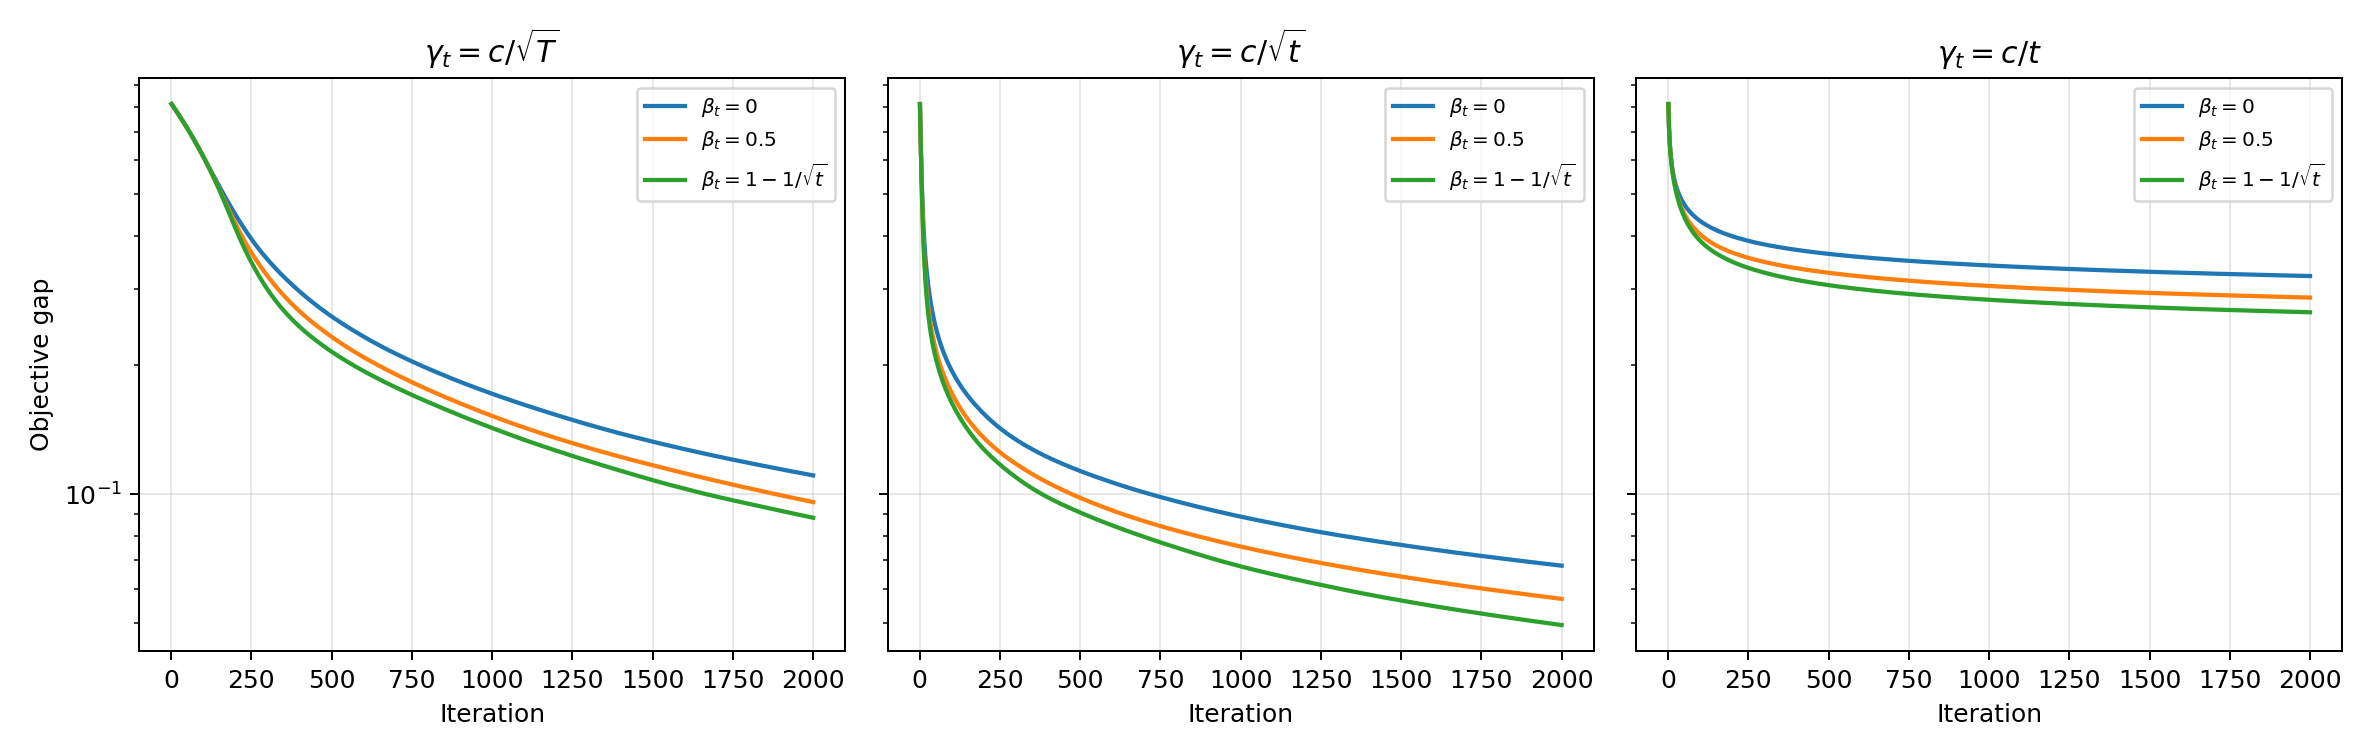
\includegraphics[width=0.98\linewidth]{../results/fig_svm_convergence.png}
    \caption{SVM schedule study: gap to the reference value}
    \label{fig:svm-convergence}
\end{figure}

\begin{figure}[H]
    \centering
    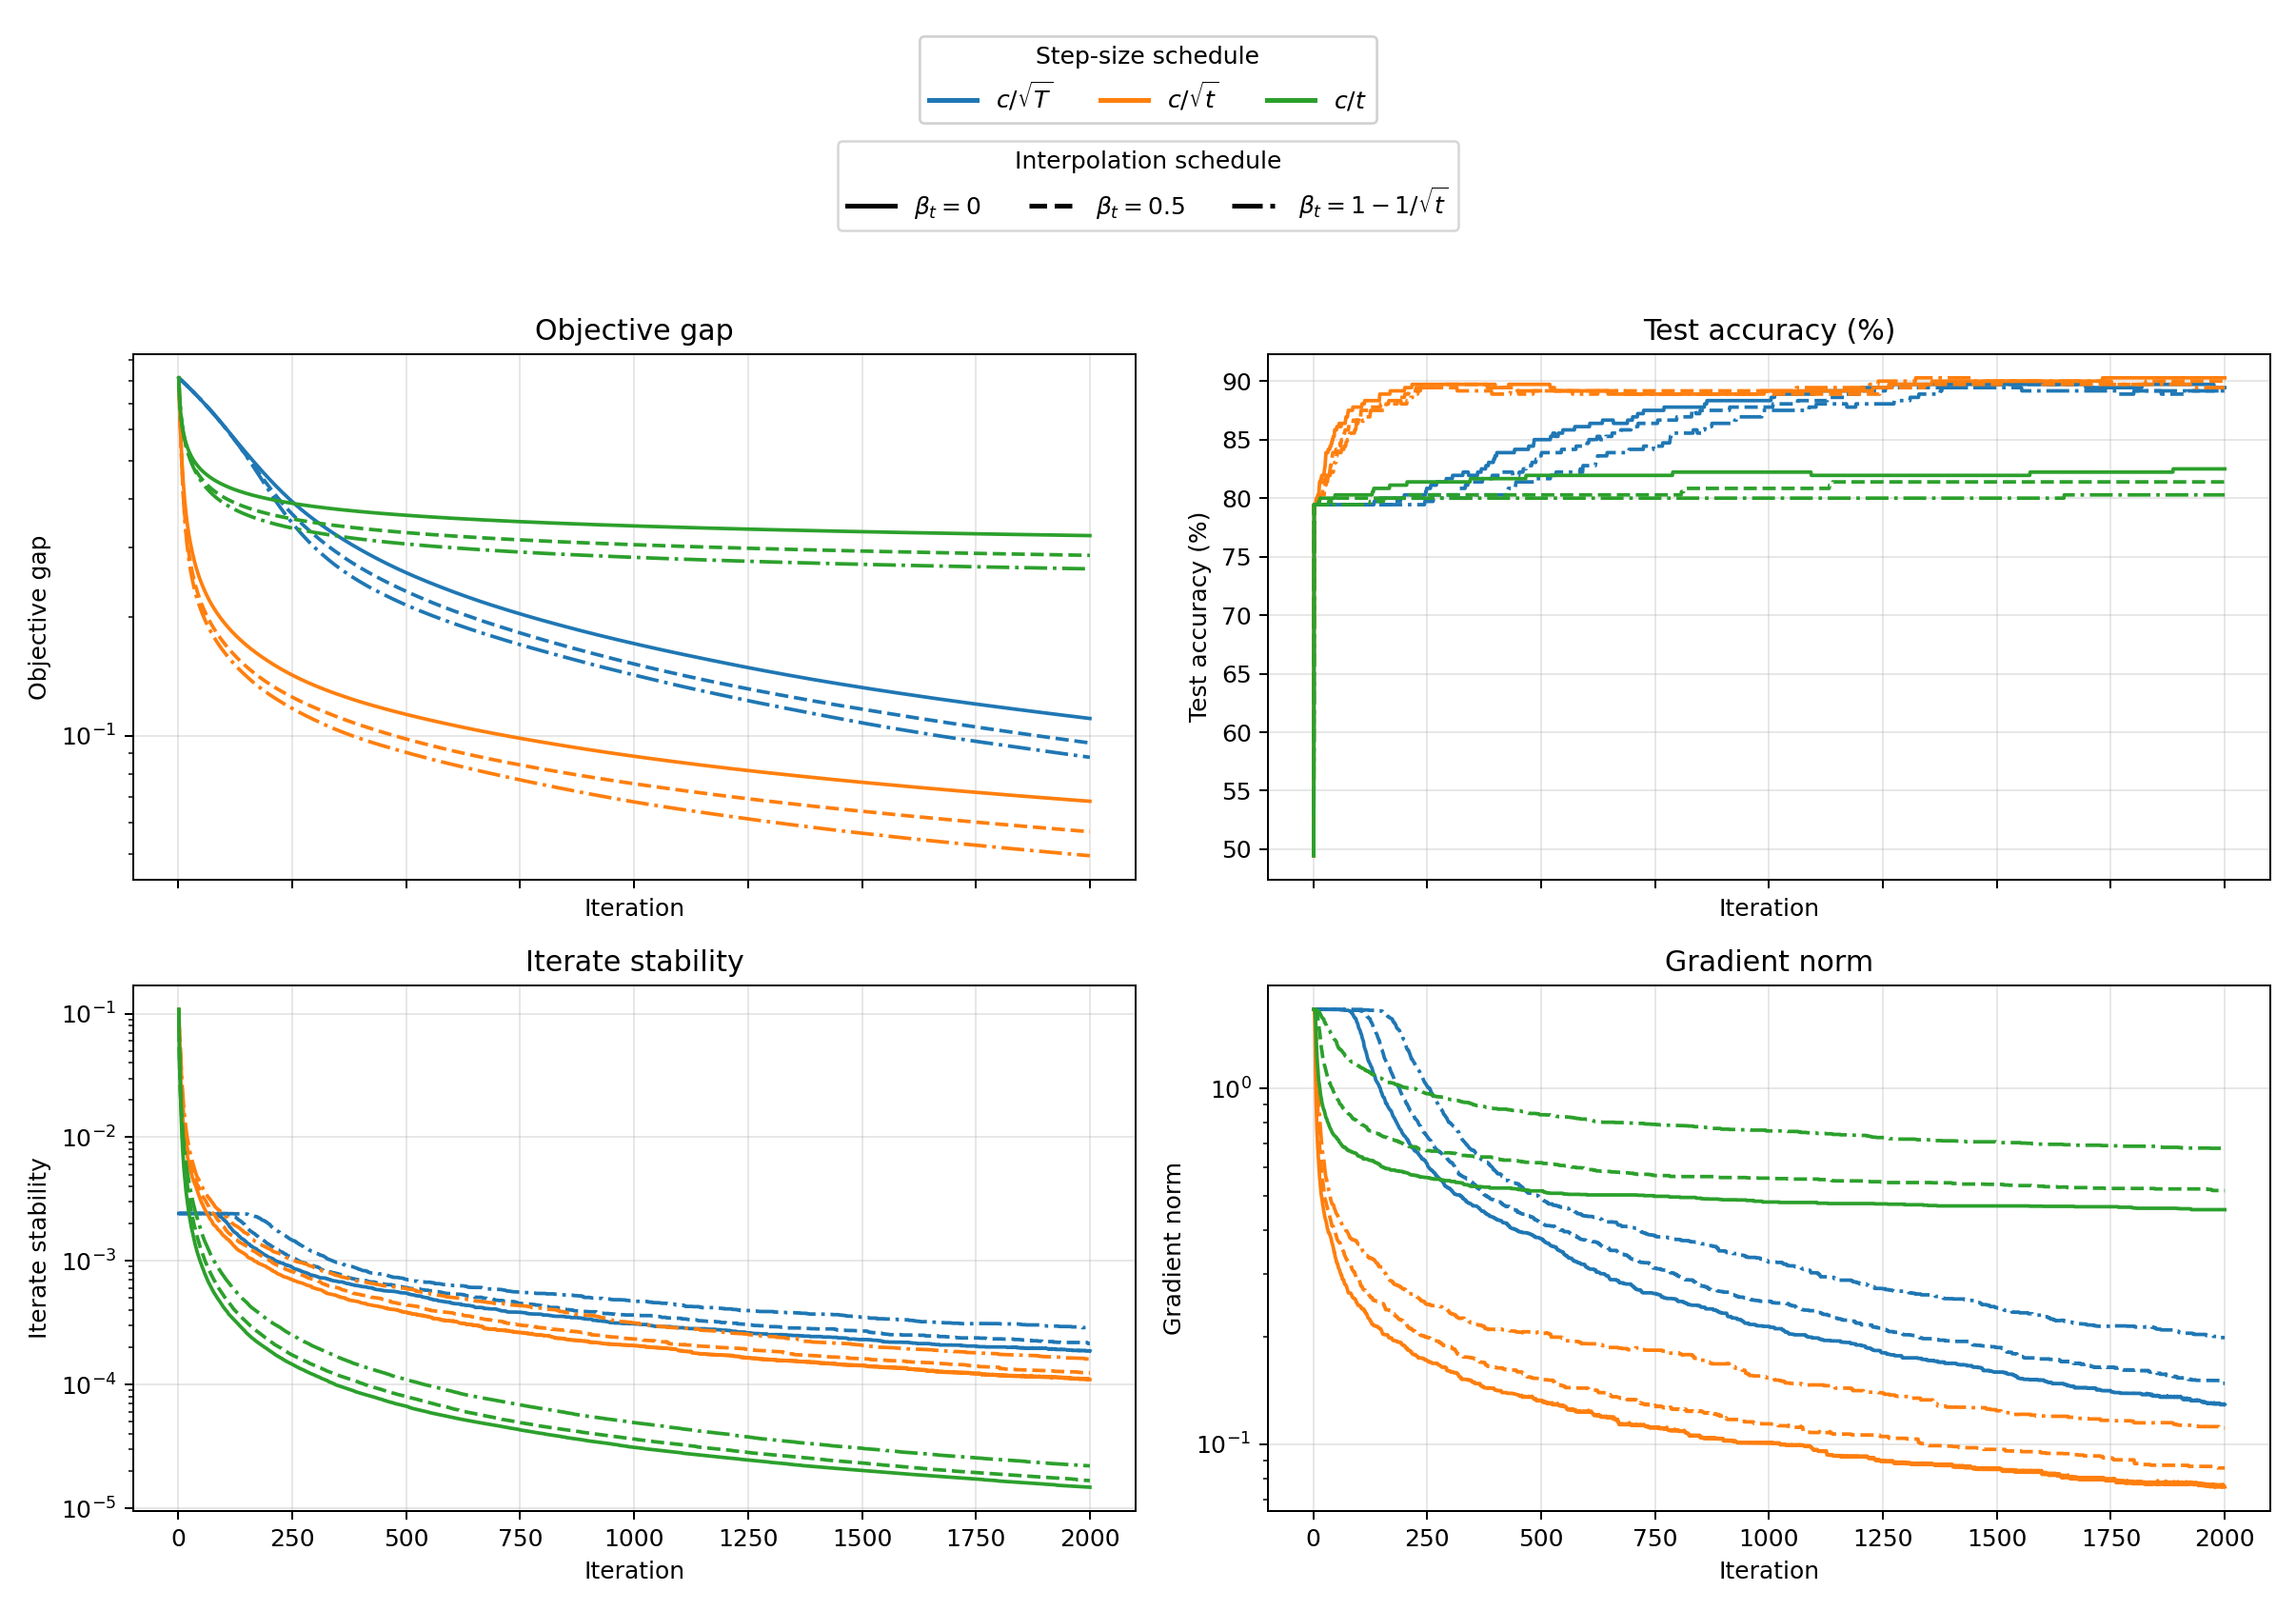
\includegraphics[width=0.98\linewidth]{../results/fig_svm_diagnostics.png}
    \caption{SVM schedule study: gap, accuracy, stability, and gradient norm}
    \label{fig:svm-diagnostics}
\end{figure}

Figure~\ref{fig:svm-convergence} and Table~\ref{tab:svm} summarize the main convergence comparison. Among the tested schedules, $\gamma_t = c/\sqrt{t}$ with $\beta_t = 1-1/\sqrt{t}$ attains the smallest final gap to the reference value, ending at final objective $0.23720$ and final gap $0.04947$. Positive interpolation reduces the final gap to the reference value for every tested averaging schedule: for $\gamma_t=c/\sqrt{T}$ the gap decreases from $0.11052$ to $0.09577$ and then to $0.08804$ as $\beta_t$ moves from $0$ to $0.5$ and then to $1-1/\sqrt{t}$; for $\gamma_t=c/\sqrt{t}$ it decreases from $0.06806$ to $0.05695$ and then to $0.04947$; for $\gamma_t=c/t$ it decreases from $0.32248$ to $0.28728$ and then to $0.26546$. Under this metric, the weakest schedule is still $\gamma_t=c/t$, whereas the highest test accuracy, $90.28\%$, is obtained by $\gamma_t=c/\sqrt{t}$ with $\beta_t=0$. The diagnostics in Figure~\ref{fig:svm-diagnostics} therefore indicate that interpolation is often helpful for the optimization metric, but not always for classification accuracy.

\begin{table}[H]
    \centering
    \caption{SVM schedule comparison}
    \label{tab:svm}
    \small
    \begin{tabular}{llllll}
        \toprule
        $\gamma_t$ & $\beta_t$ & Final obj. & Final gap & Acc. (\%) & Time (s) \\
        \midrule
        $c/\sqrt{T}$ & $0$ & 0.29826 & 0.11052 & 89.44 & 0.300 \\
        $c/\sqrt{T}$ & $0.5$ & 0.28350 & 0.09577 & 89.17 & 0.249 \\
        $c/\sqrt{T}$ & $1-1/\sqrt{t}$ & 0.27577 & 0.08804 & 89.17 & 0.245 \\
        $c/\sqrt{t}$ & $0$ & 0.25579 & 0.06806 & 90.28 & 0.280 \\
        $c/\sqrt{t}$ & $0.5$ & 0.24468 & 0.05695 & 90.00 & 0.232 \\
        $c/\sqrt{t}$ & $1-1/\sqrt{t}$ & 0.23720 & 0.04947 & 89.44 & 0.232 \\
        $c/t$ & $0$ & 0.51022 & 0.32248 & 82.50 & 0.307 \\
        $c/t$ & $0.5$ & 0.47501 & 0.28728 & 81.39 & 0.252 \\
        $c/t$ & $1-1/\sqrt{t}$ & 0.45319 & 0.26546 & 80.28 & 0.285 \\
        \bottomrule
    \end{tabular}
\end{table}

\subsection{Algorithm family comparison}
The deterministic comparison includes projected subgradient descent, dual averaging, and AdaGrad-Norm on three convex problems: hinge-loss SVM, logistic regression, and Huber regression. Projected subgradient descent uses $\gamma_t = c/\sqrt{t}$, while dual averaging and AdaGrad-Norm use constant averaging weights $\gamma_t = 1$. Dual averaging is implemented so that $x_t$ depends only on gradients observed up to time $t-1$, in accordance with the theoretical update. Each problem--algorithm pair is tuned on the pilot grid described above and is then run with the three interpolation schedules $\beta_t \in \{0,0.5,1-1/\sqrt{t}\}$.
\begin{table}[H]
    \centering
    \caption{Best deterministic configuration by problem and algorithm family}
    \label{tab:family}
    \small
    \begin{tabular}{llllll}
        \toprule
        Problem & Method & $\beta_t$ & Final obj. & Final gap & Acc. (\%) \\
        \midrule
        Huber (synthetic) & AdaGrad-Norm & $1-1/\sqrt{t}$ & 0.020198 & $6.94\times 10^{-18}$ & -- \\
        Huber (synthetic) & Dual averaging & $1-1/\sqrt{t}$ & 0.020205 & $7.00\times 10^{-6}$ & -- \\
        Huber (synthetic) & Projected subgrad. & $1-1/\sqrt{t}$ & 0.020198 & $5.66\times 10^{-13}$ & -- \\
        Logistic (digits) & AdaGrad-Norm & $0.5$ & 0.226341 & $4.20\times 10^{-5}$ & 90.28 \\
        Logistic (digits) & Dual averaging & $1-1/\sqrt{t}$ & 0.226703 & 0.00040 & 90.28 \\
        Logistic (digits) & Projected subgrad. & $0.5$ & 0.227318 & 0.00102 & 90.28 \\
        SVM (digits) & AdaGrad-Norm & $1-1/\sqrt{t}$ & 0.187753 & $2.03\times 10^{-5}$ & 91.94 \\
        SVM (digits) & Dual averaging & $1-1/\sqrt{t}$ & 0.188620 & 0.00089 & 91.67 \\
        SVM (digits) & Projected subgrad. & $1-1/\sqrt{t}$ & 0.188037 & 0.00030 & 91.94 \\
        \bottomrule
    \end{tabular}
\end{table}
Table~\ref{tab:family} lists the best configuration for each problem and algorithm under the final gap-to-reference criterion. On the Huber task, AdaGrad-Norm and projected subgradient descent nearly coincide with the reference value at final objective $0.020198$, while dual averaging ends slightly above it at $0.020205$ with gap $7.00\times 10^{-6}$. On logistic regression, AdaGrad-Norm with $\beta_t=0.5$ attains the smallest final gap to the reference value, $4.20\times 10^{-5}$, at final objective $0.226341$; dual averaging and projected subgradient descent end at $4.04\times 10^{-4}$ and $1.02\times 10^{-3}$, respectively. On the SVM task, AdaGrad-Norm with $\beta_t=1-1/\sqrt{t}$ again attains the smallest final gap to the reference value, with final objective $0.187753$ and gap $2.03\times 10^{-5}$, while projected subgradient descent and dual averaging end at $3.05\times 10^{-4}$ and $8.87\times 10^{-4}$. Figure~\ref{fig:family} confirms that these differences are much clearer in the reference-gap metric than in classification accuracy: all three methods reach $90.28\%$ on logistic regression, and on the SVM task AdaGrad-Norm and projected subgradient descent both reach $91.94\%$ while dual averaging reaches $91.67\%$.

\begin{figure}[H]
    \centering
    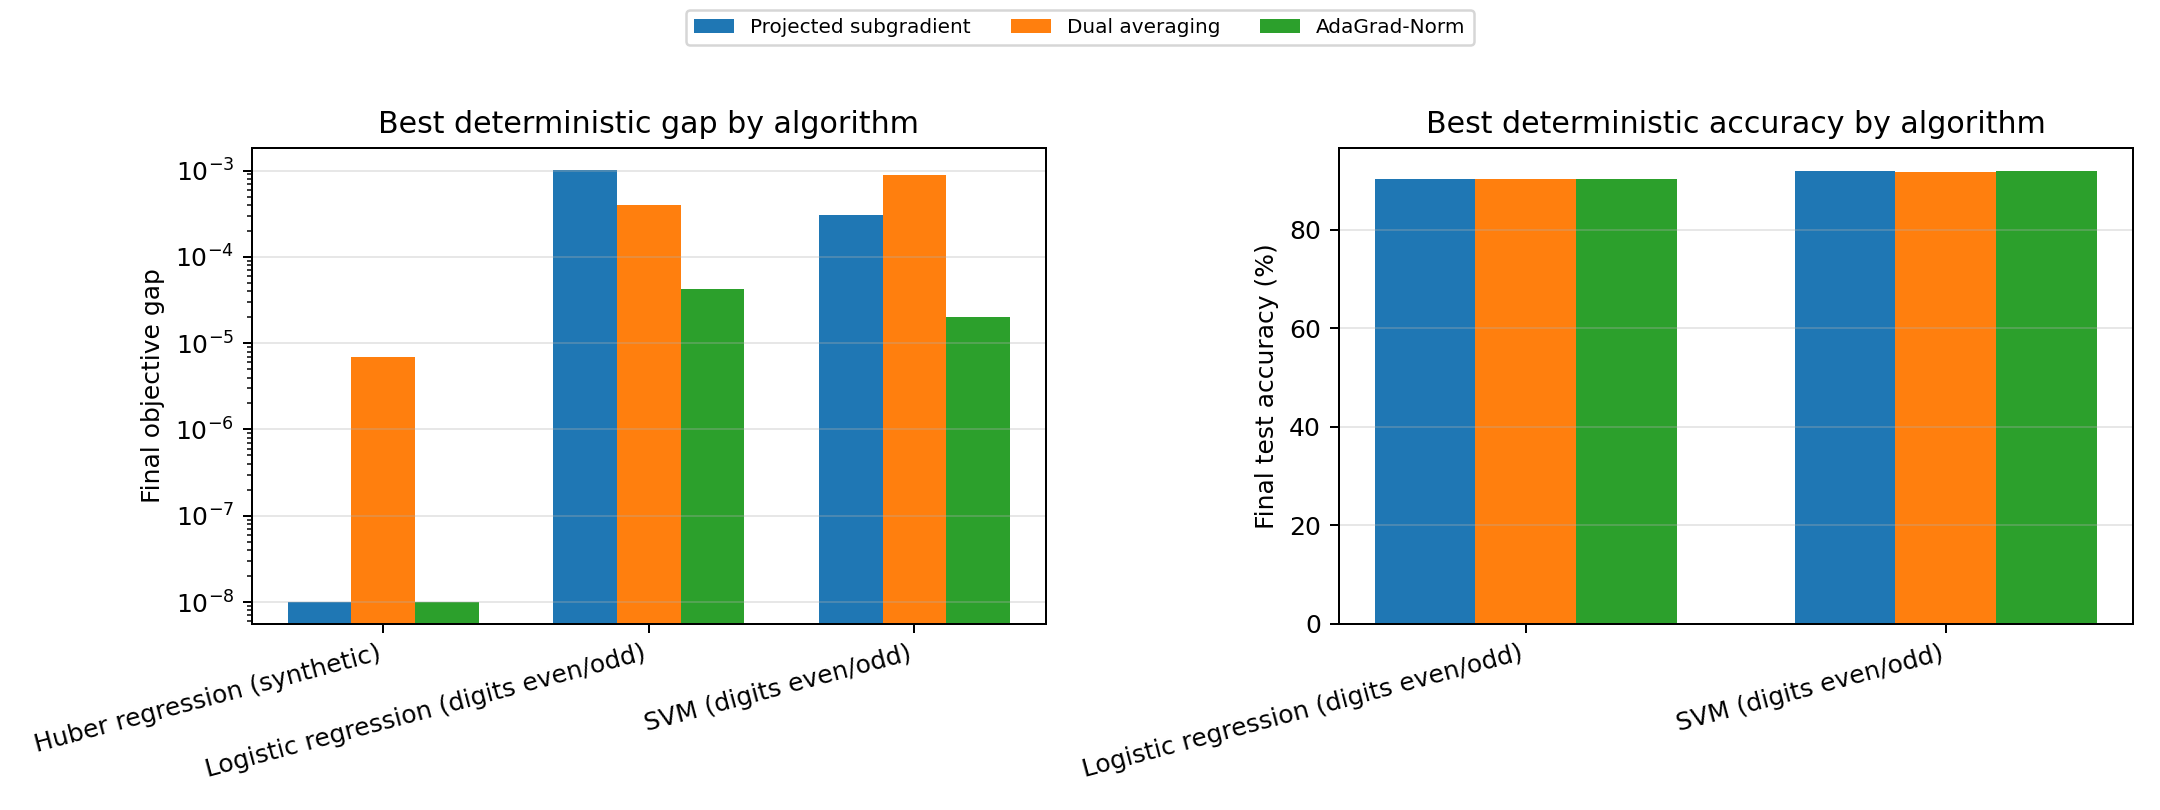
\includegraphics[width=0.92\linewidth]{../results/fig_algorithm_family_overview.png}
    \caption{Deterministic comparison across algorithm families}
    \label{fig:family}
\end{figure}


\subsection{Geometry comparison}
The geometry study isolates two settings in which non-Euclidean structure is expected to matter. The first is a simplex-constrained least-absolute-deviation problem,
\[
    \min_{w \in \Delta^{80}} \frac{1}{800}\norm{Aw-b}_1,
\]
where $A \in \R^{800 \times 80}$ has normalized columns and $b = Aw^* + \varepsilon$ with Laplace noise. The second is a logistic classification problem with $30$ coordinates whose scales grow geometrically from $10^0$ to $10^3$, together with the box constraint $[-5,5]^{30}$. On the simplex problem, Euclidean projected subgradient descent is compared to entropy mirror descent. On the ill-conditioned classification problem, Euclidean projected subgradient descent is compared to diagonal Mahalanobis mirror descent.
\begin{figure}[H]
    \centering
    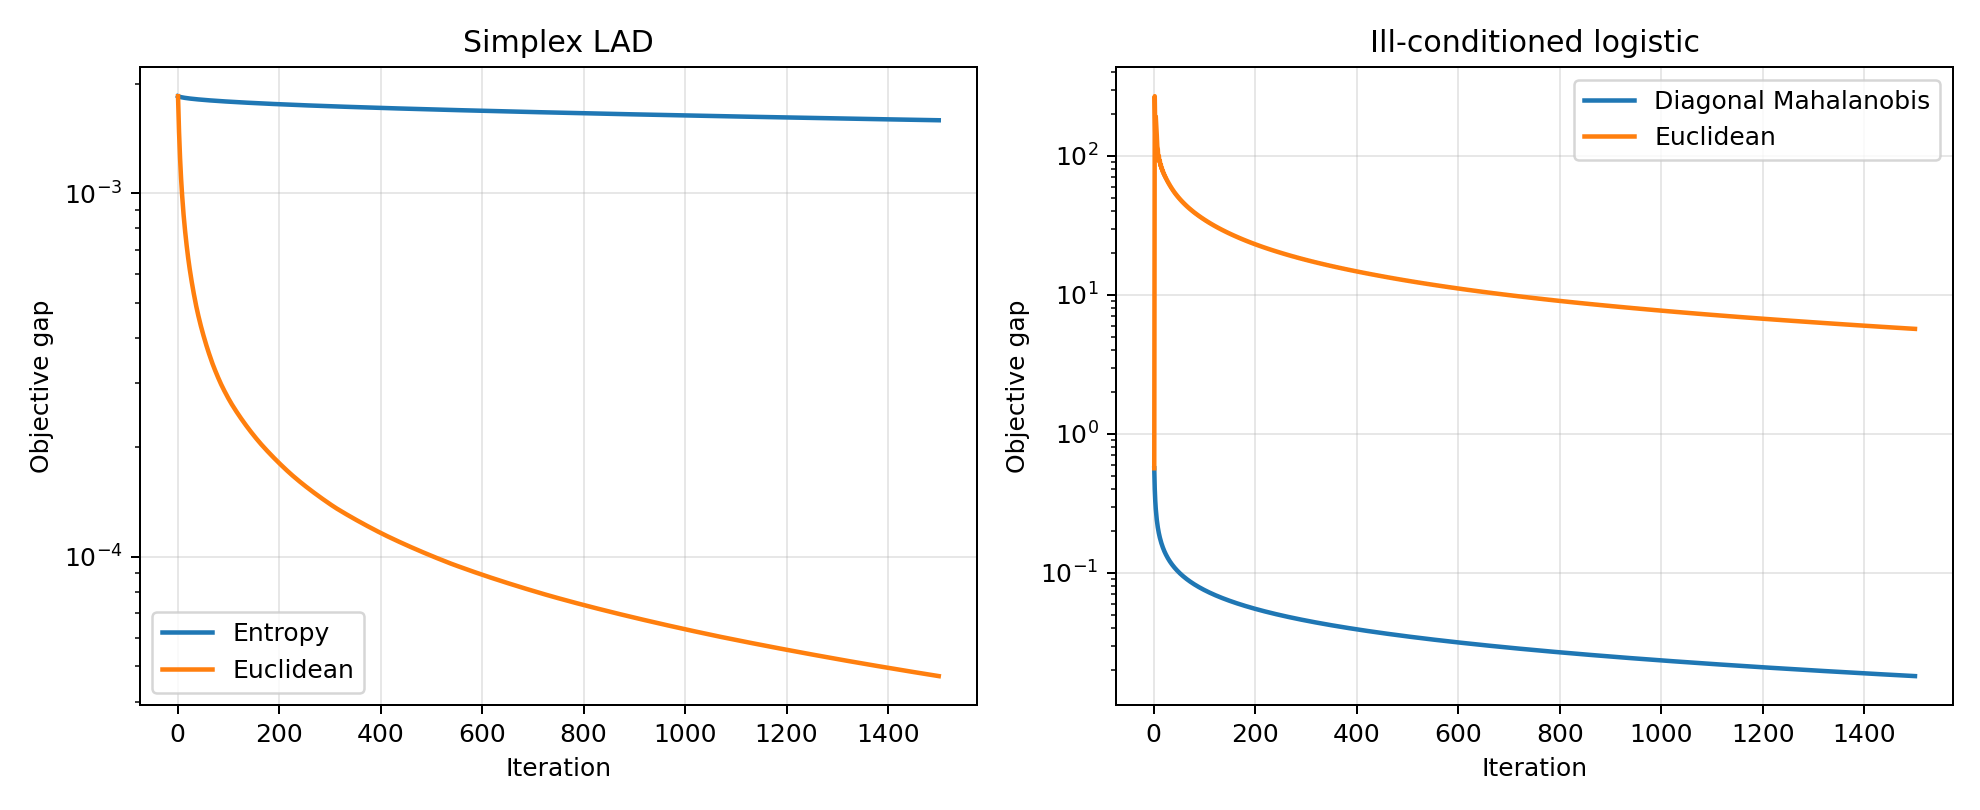
\includegraphics[width=0.92\linewidth]{../results/fig_geometry_comparison.png}
    \caption{Geometry comparison on the simplex LAD problem and the ill-conditioned logistic problem}
    \label{fig:geometry}
\end{figure}

\begin{table}[H]
    \centering
    \caption{Best configuration by geometry}
    \label{tab:geometry}
    \small
    \begin{tabular}{llllll}
        \toprule
        Problem & Geometry & Method & $\beta_t$ & Final gap & Acc. (\%) \\
        \midrule
        Simplex LAD & Entropy & Entropy MD & $0.5$ & 0.00159 & -- \\
        Simplex LAD & Euclidean & Projected subgrad. & $0.5$ & $4.70\times 10^{-5}$ & -- \\
        Ill-cond. logistic & Diag. Mahal. & Diag. Mahal. MD & $0.5$ & 0.01808 & 94.60 \\
        Ill-cond. logistic & Euclidean & Projected subgrad. & $0.5$ & 5.69307 & 83.00 \\
        \bottomrule
    \end{tabular}
\end{table}
Figure~\ref{fig:geometry} and Table~\ref{tab:geometry} summarize the geometry comparison. The effect of geometry is strongly problem dependent. On the simplex LAD benchmark, Euclidean projected subgradient descent with $\beta_t=0.5$ attains a final gap to the reference value of $4.7\times 10^{-5}$, whereas entropy mirror descent with the same interpolation level ends at $1.59\times 10^{-3}$, so the Euclidean method performs better under this metric at the tested horizon. On the ill-conditioned logistic problem, the situation reverses completely: diagonal Mahalanobis mirror descent with $\beta_t=0.5$ reaches final gap $1.81\times 10^{-2}$ and test accuracy $94.60\%$, while Euclidean projected subgradient descent remains at gap $5.69$ and accuracy $83.00\%$. The right panel of Figure~\ref{fig:geometry} makes this contrast clear, as the Mahalanobis curve continues to decrease while the Euclidean curve stalls several orders of magnitude above it.

\subsection{Stochastic experiments}
The stochastic experiments reuse the two \texttt{digits} classification tasks and compare projected subgradient descent, dual averaging, and AdaGrad-Norm under full-batch, batch-$32$, and single-sample updates. Each configuration is repeated for three random seeds. Before the interpolation sweep, each $(\text{problem}, \text{algorithm}, \text{regime})$ receives its own pilot-selected base scale from the common grid, so the comparison across regimes is not tied to a single full-batch tuning. The batch-$32$ setting is also run with additive Gaussian noise in order to separate minibatch noise from explicit gradient perturbations.

\begin{table}[H]
    \centering
    \caption{Best noisy batch-$32$ configuration for each method and problem}
    \label{tab:stochastic-noisy}
    \small
    \begin{tabular}{llllll}
        \toprule
        Problem & Method & $\beta_t$ & Mean gap & Std. gap & Acc. (\%) \\
        \midrule
        Logistic & AdaGrad-Norm & $0$ & 0.00222 & $8.99\times 10^{-5}$ & 90.00 \\
        Logistic & Dual averaging & $0.5$ & 0.00165 & 0.00011 & 90.19 \\
        Logistic & Projected subgrad. & $0.5$ & 0.00422 & 0.00016 & 89.63 \\
        SVM & AdaGrad-Norm & $0.5$ & 0.00248 & 0.00014 & 91.76 \\
        SVM & Dual averaging & $0.5$ & 0.00306 & $6.87\times 10^{-5}$ & 91.76 \\
        SVM & Projected subgrad. & $0.5$ & 0.00324 & 0.00017 & 91.48 \\
        \bottomrule
    \end{tabular}
\end{table}

Table~\ref{tab:stochastic-noisy} summarizes the noisy mini-batch results, and Figure~\ref{fig:stochastic-mean-std} displays the corresponding mean trajectories with one best configuration per method. On the logistic problem, dual averaging with $\beta_t=0.5$ attains the smallest mean final gap to the reference value in the noisy batch-$32$ regime, $1.65\times 10^{-3}$, and also the highest mean accuracy, $90.19\%$. AdaGrad-Norm with $\beta_t=0$ is second at $2.22\times 10^{-3}$, whereas projected subgradient descent with $\beta_t=0.5$ ends at $4.22\times 10^{-3}$. On the SVM problem, AdaGrad-Norm with $\beta_t=0.5$ is best under the same criterion at $2.48\times 10^{-3}$, followed by dual averaging and projected subgradient descent at $3.06\times 10^{-3}$ and $3.24\times 10^{-3}$. Figure~\ref{fig:stochastic-regimes} shows that full-batch updates remain best under this gap-to-reference metric: the smallest full-batch gaps are $3.8\times 10^{-5}$ for SVM and $8.6\times 10^{-5}$ for logistic regression, both attained by AdaGrad-Norm. The batch-$32$ regimes increase these gaps into the $10^{-3}$ range, while single-sample updates are much worse, with best gaps of $4.85\times 10^{-2}$ on SVM and $2.80\times 10^{-2}$ on logistic regression. At the calibrated perturbation level, the extra Gaussian noise does not materially worsen the batch-$32$ results and is slightly favorable for several methods, so the dominant degradation comes from sampling noise rather than from the explicit perturbation itself.

\begin{figure}[H]
    \centering
    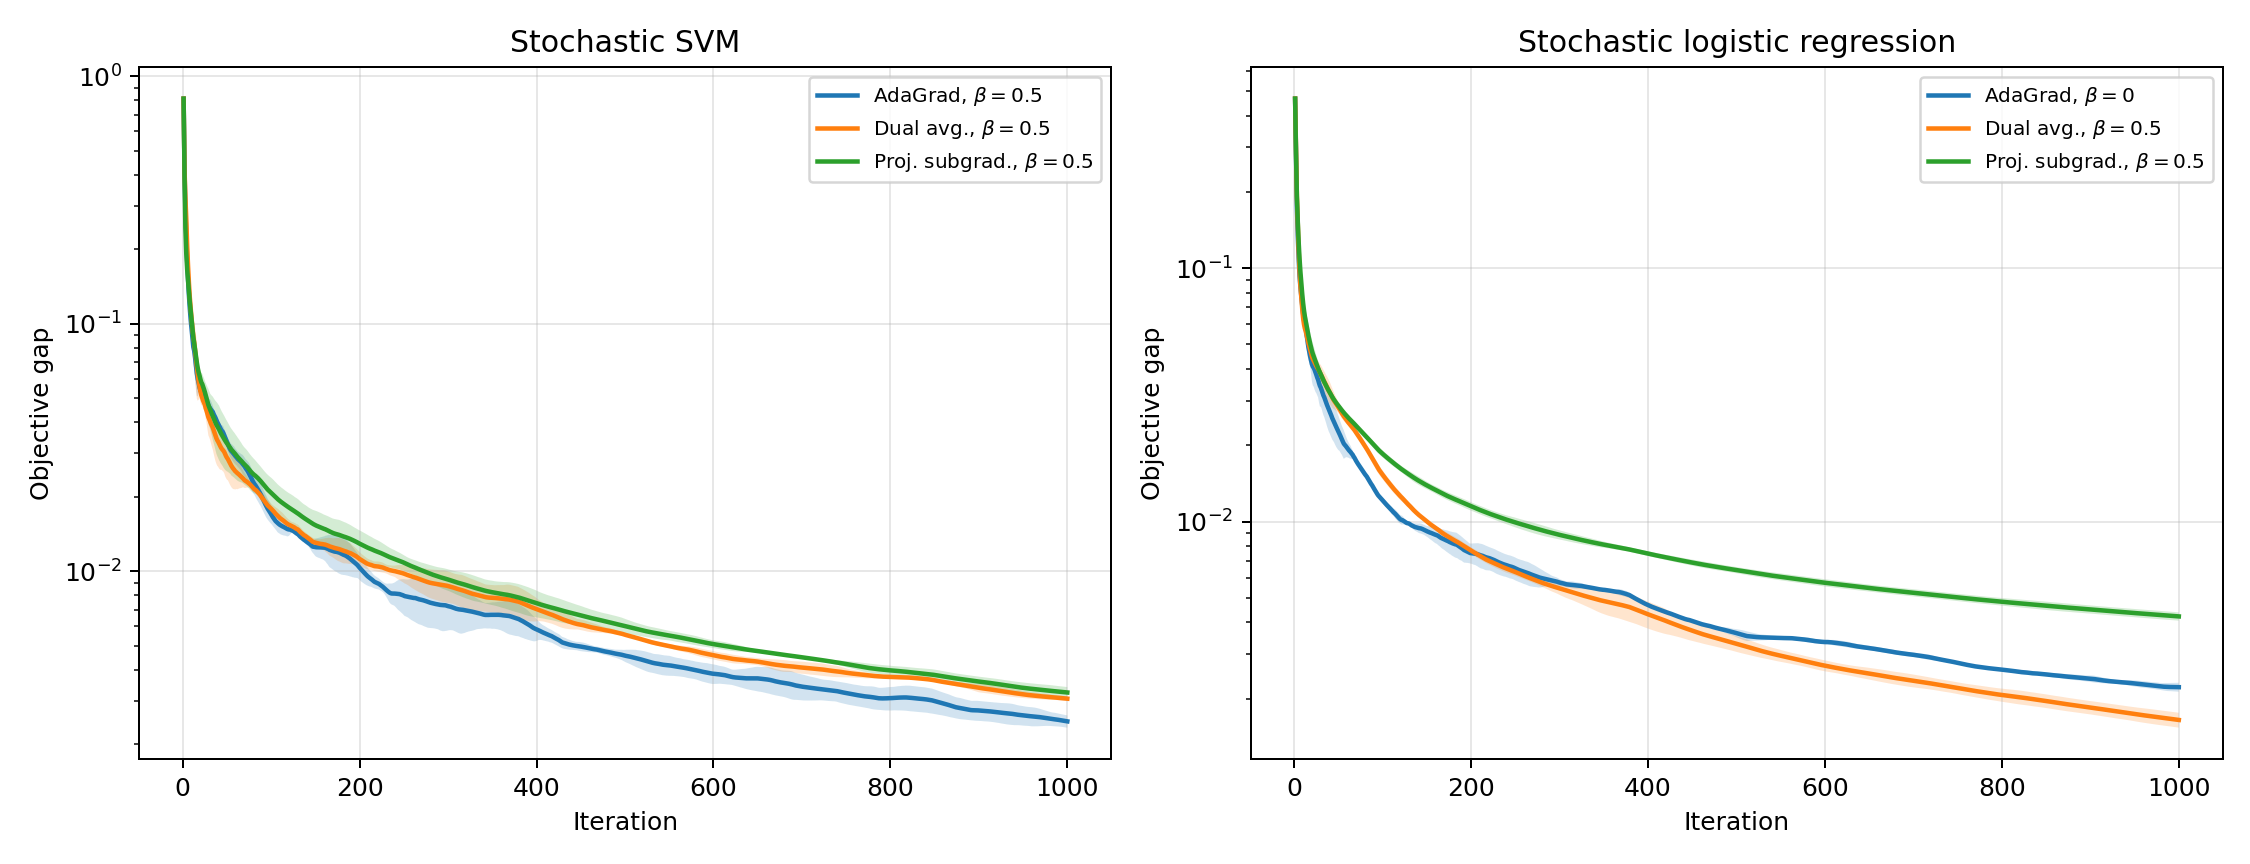
\includegraphics[width=0.98\linewidth]{../results/fig_stochastic_mean_std.png}
    \caption{Stochastic experiments on the digits tasks: mean and standard deviation in the noisy batch-$32$ setting}
    \label{fig:stochastic-mean-std}
\end{figure}

\begin{figure}[H]
    \centering
    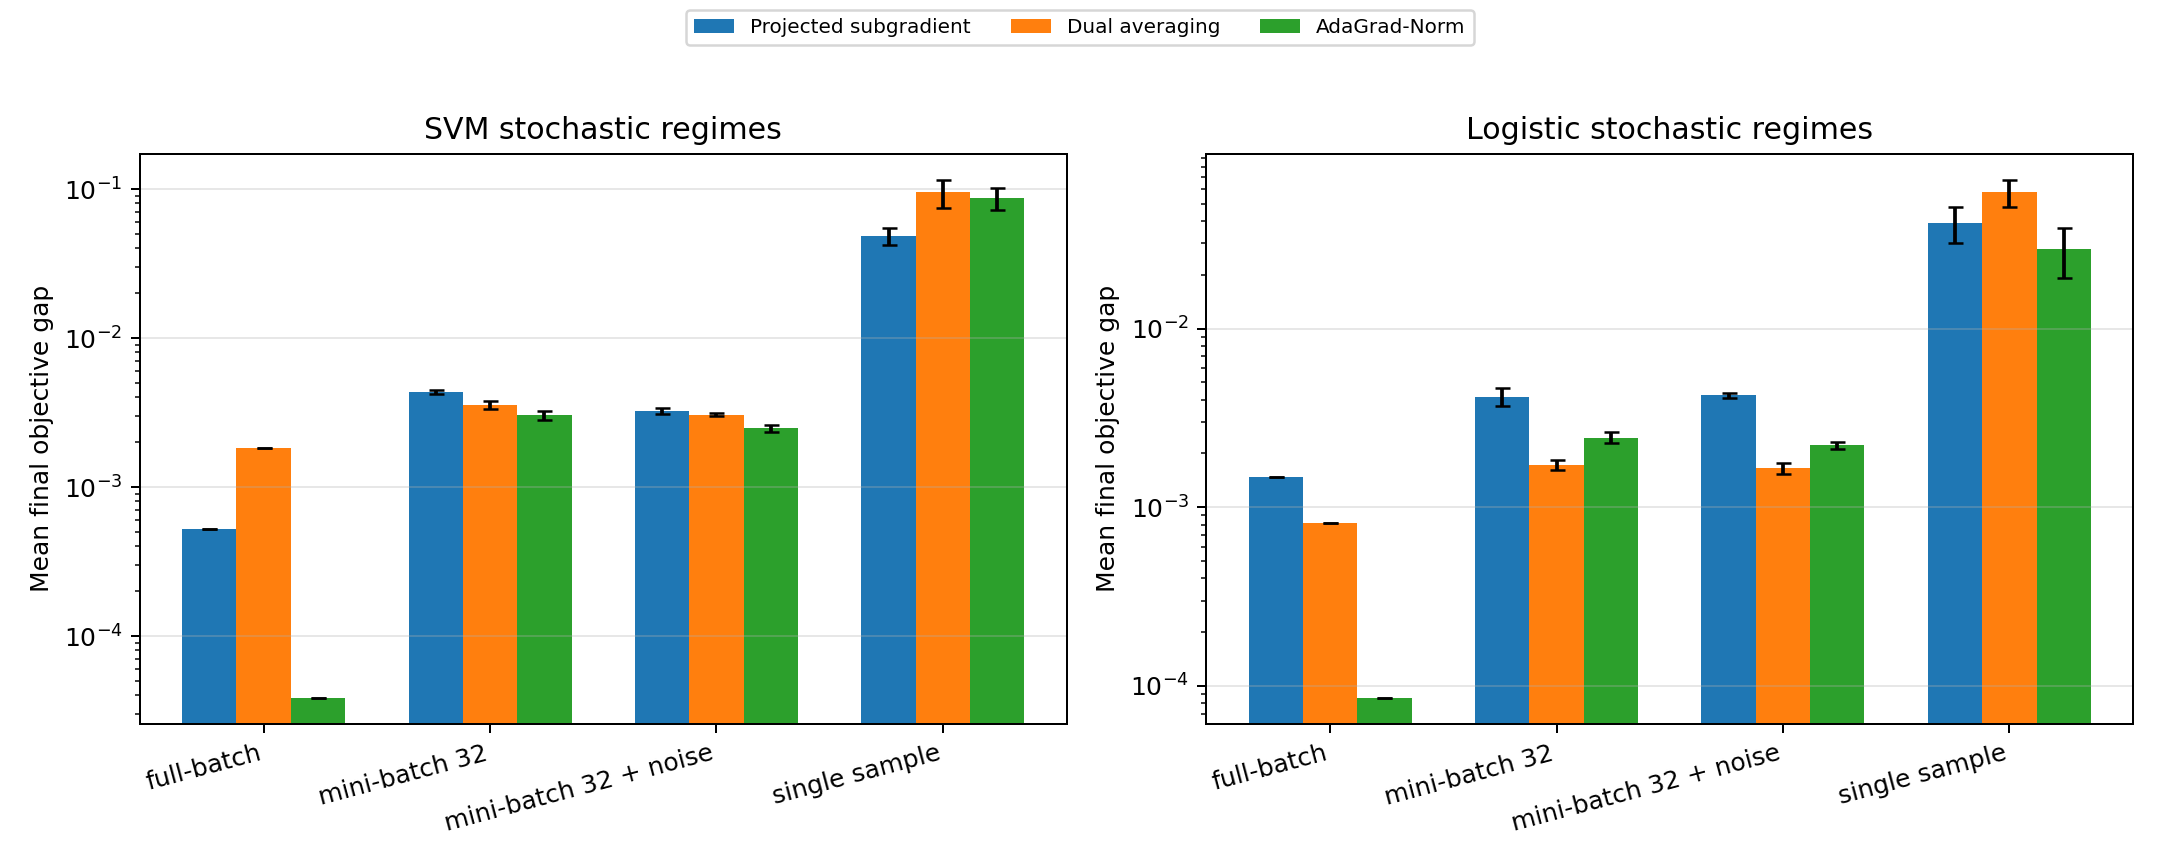
\includegraphics[width=0.98\linewidth]{../results/fig_stochastic_regimes.png}
    \caption{Stochastic experiments on the digits tasks: best mean final gap to the reference value by stochastic regime}
    \label{fig:stochastic-regimes}
\end{figure}

\subsection{Results and discussion}
Taken together, these experiments support four main conclusions. First, interpolation is consistently helpful for the reported optimization metric in the SVM schedule study, but there is no universally optimal $\beta_t$: the preferred interpolation level varies across problems and algorithms, and the schedule with the smallest final gap to the reference value need not be the one with the highest test accuracy. Second, among the three Euclidean algorithm families, AdaGrad-Norm is the strongest method on the two classification problems under the reference-gap metric and is effectively tied with projected subgradient descent on the Huber task. Third, geometry matters most under poor conditioning: entropy geometry is not helpful on the tested simplex benchmark, whereas diagonal Mahalanobis geometry yields an improvement of more than two orders of magnitude on the ill-conditioned logistic problem. Fourth, at the tested perturbation level, stochastic degradation is driven mainly by small-batch sampling rather than by the added Gaussian noise. Full-batch updates remain best in objective value, batch size $32$ preserves much of the performance, and single-sample updates degrade sharply.

\section{Conclusion}
The report studies a generalized weighted-averaging scheme for nonsmooth convex optimization from both analytical and numerical perspectives. The analysis shows that evaluating subgradients at the interpolation point $z_t$ still leads to clean objective bounds for mirror descent, projected subgradient descent, dual averaging with time-dependent parameters, and AdaGrad-Norm once performance is measured at the weighted average $\bar{x}_T$. The experiments indicate that interpolation is often beneficial for the reported gap-to-reference metric, but its effect depends on the problem class, the update rule, the noise regime, and the underlying geometry.

\end{document}
